\subsection{Parameterisation of Animation}
\label{sec:Param}

What we mean by \emph{parameterisation} is the ability, for an AU, to separate 
the internal animation logic so that it becomes possible to apply it consistently
to elements from different \DSLs, thus promoting reuse. Taking our \DSLs of \S 
\ref{sec:Examples}, we see that \textsf{PM.1}, \textsf{FSM.2.1} and \textsf{PN.3.1}
all involve the same animation logic (\emph{disappear} from the current location, 
followed by \emph{appear} on another location), but applied to different elements:
in \textsf{PM}, it concerns the \textsf{Persona}; in \textsf{FSM}, it concerns the
\textsf{Token}; and in \textsf{PN}, it iteratively applies to the markings.

The exact mechanism required for implementing this feature into MA is beyond this
paper's scope. However, there is essentially two ways to realise it:
\begin{description}
   \item[Using model's elements] The first one consists of explicitly referencing
   the model's elements (either objects or links). Retrieving the corresponding 
   graphical elements can be achieved through the mapping to the CS. This approach
   has the advantage of directly reusing the models, preventing MA designers from
   any extra work. However, the task may be complicated by the presence of complex
   rendering patterns that need to be computed before determining which graphical
   object the AU logic applies to.
   
   \item[Using the graphical elements] The second, and opposite approach consists
   of directly referencing the graphical elements impacted by an AU. In this case,
   the UA does not depend on the complexity of rendering patterns, but has the 
   drawback of preventing to easily retrieve which elements in the model have been
   impacted by an animation.
\end{description}

\autoref{fig:UA-Param} shows how parameters could be integrated into animations. 
Two basic animation units \textsf{APP} (making an element appear) and \textsf{DAPP}
(making an element disappear) with their respective parameters. They are then
composed into a complex unit \textsf{BLINK}, which exposes the parameters of
the previous units and adds a new one for controlling the blinking delay.

\begin{figure}[t]%
   \centering
   %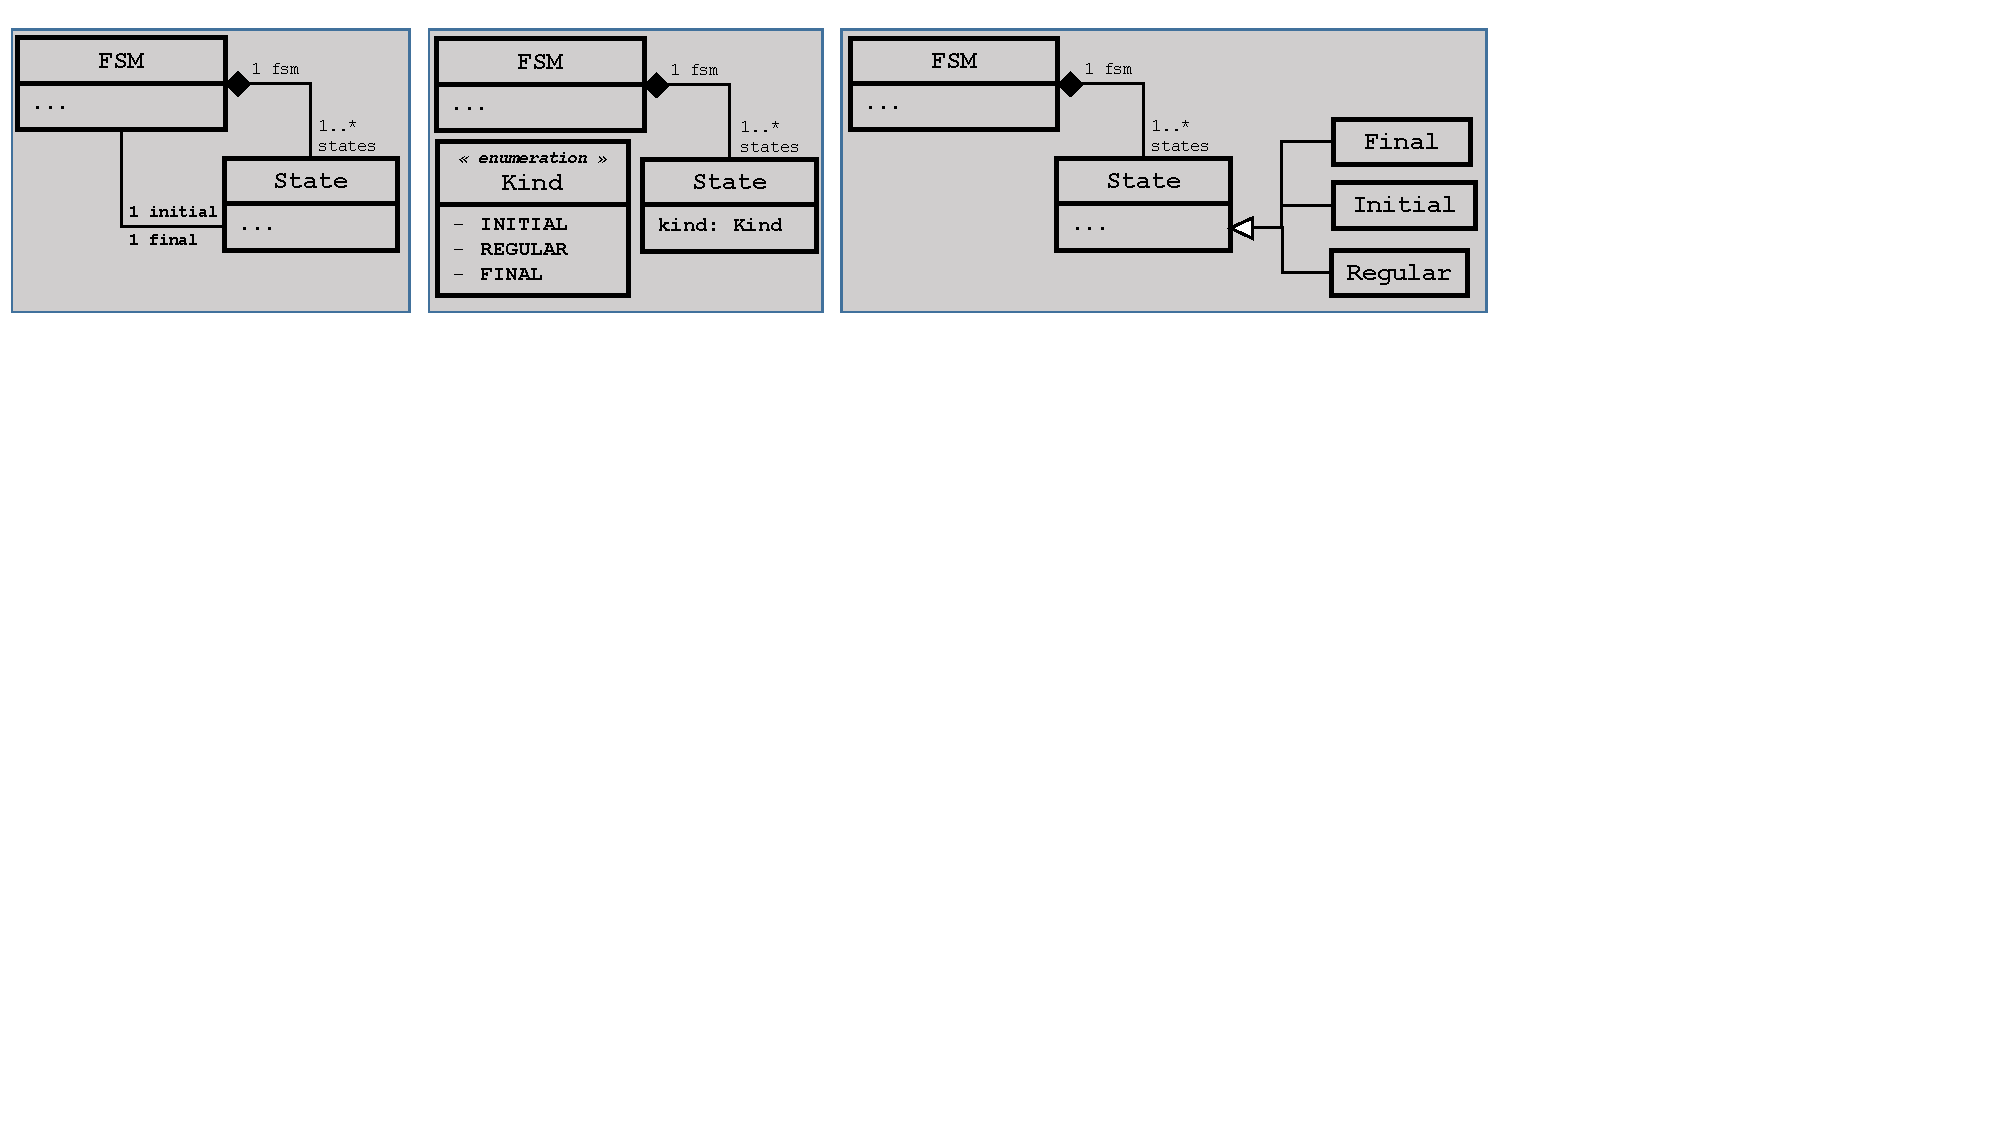
\includegraphics[width=\columnwidth,clip, trim=0cm 13.8cm 8.3cm 0.2cm]{FSM-Initial}%
   \caption{Two basic AUs: \textsf{APP} and \textsf{DAPP} with their parameters;
   and a possible combination to create a complex unit \textsf{BLINK}.
   }%
   \label{fig:UA-Param}%
\end{figure}